\chapter{Baggrund} \label{chap:Baggrund}

Apopleksi (pludseligt opstået fokale neurologiske symptomer) opstår af infarkt eller en blødning. Ved infarkt nedsættes eller afbrydes blodforsyningen i visse område af hjernen og dette medfører iltmangel i det ramte område. I 85\% af tilfælde er apopleksi forårsaget af infarkt og 15\% skyldes blødning \fixme{Reference til "Basis i sygdomslære, side 399-402}

Hvert år indlægges ca. 12.000 danskere i forbindelse med apopleksi og i den vestlige verden er apopleksi det tredjehyppigste dødsårsag.\fixme{Reference program apopleksi, side 14}. Af de personer der overlever et apopleksi tilfælde, lever næsten 50\% af dem med varige men og 25\% af dem har behov for andres hjælp ved daglige aktiviteter. \fixme{Refence til fakta om apopleksi http://www.hjernesagen.dk/om-hjerneskader/bloedning-eller-blodprop-i-hjernen/fakta-om-apopleksi } Det høje antal tilfælde årligt og de mange personer med varige men har store omkostninger for sundhedssektoren.  I 2001 kostede apopleksi sundhedsvæsnet 1,8 milliarder kroner. \fixme{Reference til trombolyse økonomi side 17}

Den nuværende behandling af apopleksi og dets følgevirkning sker i flere forskellige trin; forbyggende, akut behandling og rehabilitering. 

Meget af den forebyggende behandling af apopleksi ligger i livstilsændringen. Faktorer for udvikling af apopleksi er bl.a. hypertension, hjerte-kar sygdomme, arteriosklerose og forhøjet kolesterol. 

For at opnå størst effekt af akut behandling af apopleksi skal behandlingen helst ske inden for 5 timer efter tilfældet indtræf. Behandlingen består som regel af en scanning for afgøre om der er tale om en blodprop eller en blødning. Hvis der er tale om en blodprop, vil patienten modtage trombolysebehandling 

Afhængig af méngraden består rehabiliteringen af genoptræning i forskellige form. Menene af apopleksi kan være alt fra talebesvær til halvsidig lammelse og derfor afhænger genoptræning også deraf. \fixme{https://www.sundhed.dk/borger/sygdomme-a-aa/hjerte-og-blodkar/sygdomme/apopleksi/behandling-ved-apopleksi/}

\section{noninvasiv blodtryksmåling}\label{noninvasivBloodpressureMeasurement}
Noninvasiv blodtryksmåling, eller indirekte måling af det arterielle blodtryk er fællesbetegnelsen, for flere typer af tekniker, som alle estimerer blodtrykket i arteriet. Ofte associeres en blodtryksmåling af denne type, med den manuelle auditive detektion af puls, distal til en okkluderende manchet, som kan ses på figur \ref{fig:audiotoryBloodpressureMeasurement}). Denne manuelle auskulatoriske metode med kviksølvs sphygmomanometer anses stadig for at være guldstandarden inden for noninvasiv blodtryksmonitorering.\fixme{Requirements for professional office blood pressure monitors}

\begin{figure}[H]
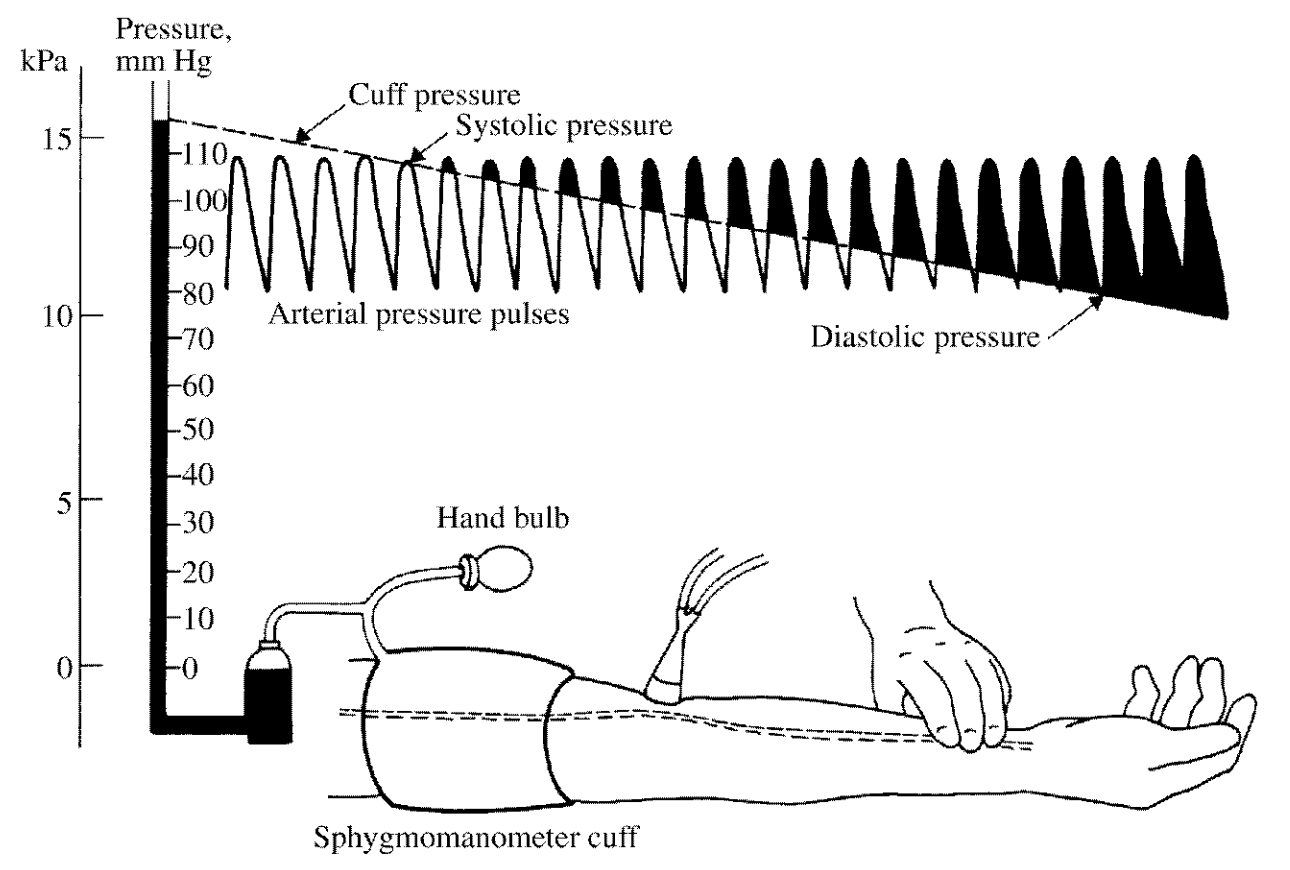
\includegraphics[width=0.9\textwidth]{billeder/TypicalIndirectBlood-pressureMeasurement.png}
\caption{Typisk indirekte blodtryksmåling med sphygmomanometer, manchet ogstetoskop}\label{fig:audiotoryBloodpressureMeasurement}
\end{figure}
\fixme{ref: Webster side 325}

Det automatiske blodtryks apparat som erstatter den manuelle auditive metode (automatiseret auskultatorisk apparat) anvender i alt sin simpelhed en mikrofon i stedet for stetoskopet. Ultralyd anvendes også i nogle blodtryksapparater som erstatning af stetoskoppet og bestemmer ved hjælp af doppler, hvornår arteriet er total okkluderet af manchetten. Ultralyd har særlige fordele, så som at kunne bruges på spædbørn og hypotensive patienter, hvor lyden af blodflowvibrationerne i arteriet kan være svære at hører. Langt de fleste blodtryksmållere anvender dog i dag den oscillometriske metode, hvor selve manchetten selv agerer som interface til det pulserende arterie (se figur \ref{fig:OscillometriskMetode}).\fixme{Requirements for professional office blood pressure monitors} Det ekspanderende arterie skubber til manchetten og skaber oscilloerende trykændringer i manchetten. På samme måde, som ved den auskultatoriske metode pumpes trykket i manchetten til over systolisk blodtryk, hvor arteriet er total okkluderet og manchetten udsættes på dette stadie ikke for pulsationer fra det underlæggene arterie. Luften i manchetten lukkes gradvist ud over tid. Når arterie trykket overstiger manchet trykket løber blodet ind i arteriet og skubber til arterievæggen. De små oscillotioner overføres til manchetten, hvilket resulterer i trykændringer (de største trykændringer i manchetten kan også observeres i sphygmomanometeret under en auskulatorisk måling). Oscillotionerne isoleres fra manchetrykket og kan ses på figur \ref{fig:OscillometriskMetode}. Middel arterie trykket ses hvor oscillotionerne er størst og det systoliske blodtryk ses hvor en pludseligt stigning i amplitude højden finder sted. Diastolen har ikke en klar overgang og er derfor bestemt ud fra algoritmer.\fixme{Webster side 328}

\begin{figure}[H]
	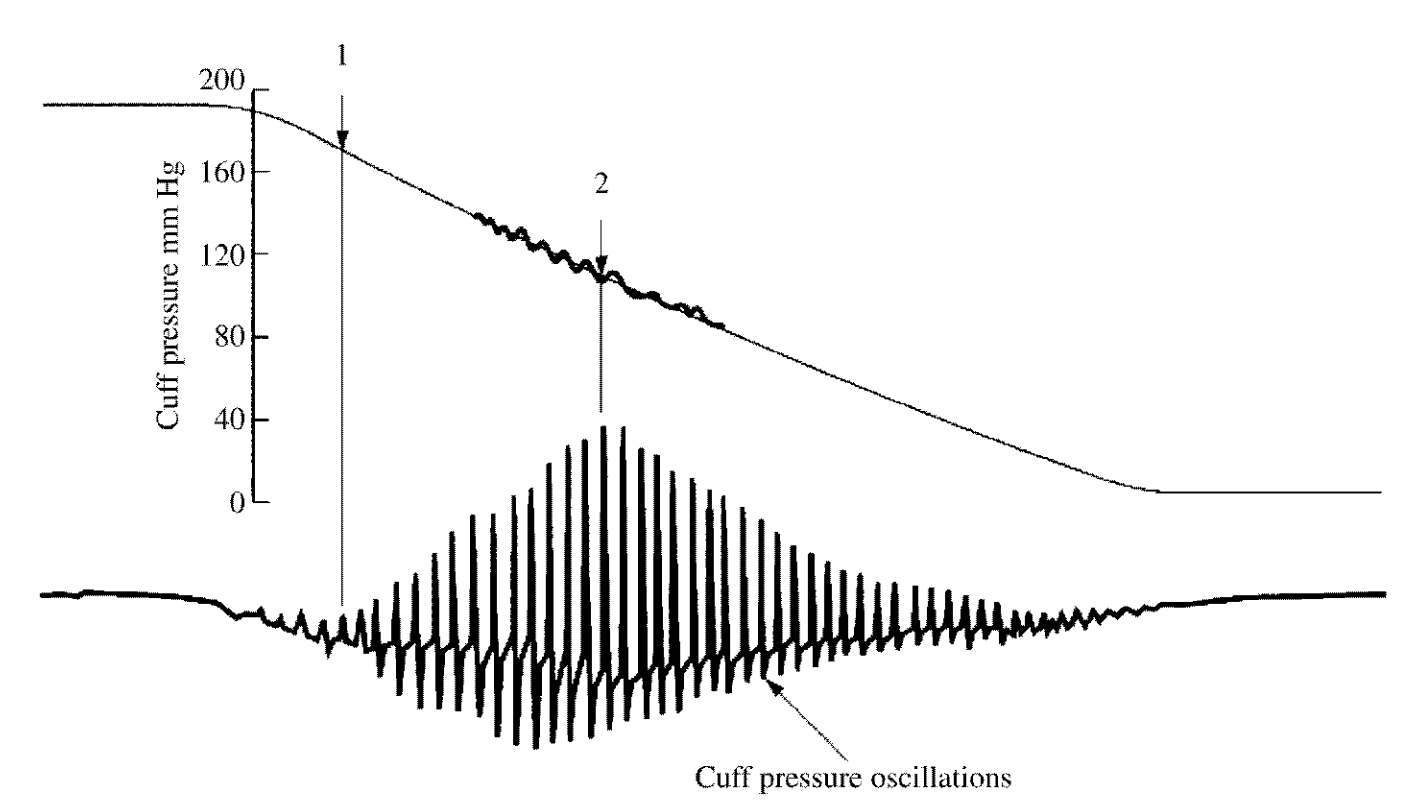
\includegraphics[width=0.9\textwidth]{billeder/OscillometriskMetode.png}
	\caption{Den oscillometriske metode. En kompressionsmanchet oppustes til et tryk over det systolisk blodtryk. Luften lukkes langsomt ud, hvorefter det systoliske tryk måles ved punkt 1 og MAP ved punkt 2. Det systoliske tryk ses ved den pluslige stigning i de oscillostionernes ampletuder og MAP er manchettrykket ved de største oscillotioner er til stede.}\label{fig:OscillometriskMetode}
\end{figure}
\fixme{ref: Webster side 329}

\section{Konditionering}









